\everymath{\displaystyle}
\documentclass{beamer}
% \documentclass[handout]{beamer}

%\usepackage[pdftex]{color,graphicx}
\usepackage{amsmath,amssymb,amsfonts}

\mode<presentation>
{
  % \usetheme{Darmstadt}
  % \usetheme[hideothersubsections]{Hannover}
  % \usetheme[hideothersubsections]{Goettingen}
  \usetheme[hideothersubsections, right]{Berkeley}

  \usecolortheme{seahorse}
  % \usecolortheme{dolphin}
  \usecolortheme{rose}
  % \usecolortheme{orchid}

  \useinnertheme[shadow]{rounded}

  \setbeamercovered{transparent}
  % or whatever (possibly just delete it)
}

\mode<handout>{
  \setbeamercolor{background canvas}{bg=black!5}
  \usepackage{pgfpages}
  \pgfpagesuselayout{4 on 1}[a4paper,border shrink=5mm, landscape]
}

\usepackage[brazilian]{babel}
% or whatever

% \usepackage[latin1]{inputenc}
\usepackage[utf8]{inputenc}
% or whatever

\usepackage{times}
%\usepackage[T1]{fontenc}
% Or whatever. Note that the encoding and the font should match. If T1
% does not look nice, try deleting the line with the fontenc.


\title%[] % (optional, use only with long paper titles)
{Testes de Hipóteses I}

\subtitle
{Testes para uma amostra} % (optional)

\author%[] % (optional, use only with lots of authors)
{Felipe Figueiredo}% \and S.~Another\inst{2}}
% - Use the \inst{?} command only if the authors have different
%   affiliation.

\institute[INTO] % (optional, but mostly needed)
{Instituto Nacional de Traumatologia e Ortopedia
}
  % \inst{1}%
  % Department of Computer Science\\
  % University of Somewhere
  % \and
  % \inst{2}%
  % Department of Theoretical Philosophy\\
  % University of Elsewhere}
% - Use the \inst command only if there are several affiliations.
% - Keep it simple, no one is interested in your street address.

\date%[] % (optional)
{}

% \subject{Talks}
% This is only inserted into the PDF information catalog. Can be left
% out. 



% If you have a file called "university-logo-filename.xxx", where xxx
% is a graphic format that can be processed by latex or pdflatex,
% resp., then you can add a logo as follows:

\pgfdeclareimage[height=1.6cm]{university-logo}{../logo}
\logo{\pgfuseimage{university-logo}}



% Delete this, if you do not want the table of contents to pop up at
% the beginning of each subsection:
\AtBeginSubsection[]
%\AtBeginSection[]
{
  \begin{frame}<beamer>{Sumário}
    \tableofcontents[currentsection,currentsubsection]
  \end{frame}
}


% If you wish to uncover everything in a step-wise fashion, uncomment
% the following command: 

\beamerdefaultoverlayspecification{<+->}


\begin{document}

\begin{frame}
  \titlepage
\end{frame}

\begin{frame}{Sumário}
  \tableofcontents
  % You might wish to add the option [pausesections]
\end{frame}


%% Template
% \section{}

% \subsection{}

% \begin{frame}{}
%   \begin{itemize}
%   \item 
%   \end{itemize}
% \end{frame}

% \begin{frame}
%   \begin{columns}
%     \begin{column}{5cm}
%     \end{column}
%     \begin{column}{5cm}
%     \end{column}
%   \end{columns}
% \end{frame}

% \begin{frame}{}
%   \includegraphics[height=0.4\textheight]{file1}
%   \includegraphics[height=0.4\textheight]{file2}
%   \includegraphics[height=0.4\textheight]{file3}
%   \begin{figure}
%     \caption{}
%   \end{figure}
% \end{frame}

% \begin{frame}{}
%   \begin{definition}
%   \end{definition}
%   \begin{example}
%   \end{example}
%   \begin{block}{Exercício}
%   \end{block}
% \end{frame}

\section{Testes de Hipóteses}

\begin{frame}{Testes de Hipóteses}
  \begin{itemize}
  \item Podemos tomar decisões baseado nos dados de um experimento
    (amostra).
  \item Para isto, precisamos de um critério sistemático e rigoroso
    que possa aferir o quanto os dados suportam esta decisão.
  \item Usando os conceitos de probabilidades, poderemos ainda
    calcular a probabilidade de que esta decisão esteja errada.
  \end{itemize}
\end{frame}

\begin{frame}{Testes de Hipóteses}
  \begin{definition}
    Em Estatística, uma \alert{hipótese} é uma afirmação sobre uma
    característica de uma população, tipicamente o valor de um
    parâmetro.
  \end{definition}
  \begin{definition}
    Um \alert{teste de hipótese} (ou teste de significância) é um
    procedimento sistemático para testar uma afirmação sobre uma
    característica de uma população.
  \end{definition}
\end{frame}

\begin{frame}{Componentes de um testes de hipóteses}
  São necessários para um teste de hipóteses:
  \begin{itemize}
  \item As hipóteses nula e alternativa
  \item O nível de significância
  \item A estatística de teste
  \item A região crítica
%  \item 
  \end{itemize}
\end{frame}

\subsection{Hipóteses}

\begin{frame}{Identificando hipóteses}
  \begin{itemize}
  \item Uma hipótese estatística deve ser testável frente a dados
    obtidos de um experimento.
  \end{itemize}
  \begin{example}
    Um jornalista alega que a maior parte dos motoristas atravessa o
    sinal vermelho.
  \end{example}
  \begin{example}
    Pesquisadores afirmam que a temperatura corporal média de adultos
    sadios não ultrapassa 37$^o$C.
  \end{example}
\end{frame}

\begin{frame}{Identificando hipóteses}
  \begin{itemize}
  \item Para efetuar um teste de hipóteses é necessária a formulação
    de uma \alert{hipótese nula} e uma \alert{hipótese alternativa}.
  \item A hipótese nula ($H_0$) é uma hipótese que contém uma
    afirmação de igualdade.
  \item A hipótese alternativa ($H_1$ ou $H_a$) é o complementar da
    hipótese nula.
  \end{itemize}
\end{frame}

\begin{frame}{Identificando hipóteses}
  \begin{block}{Atenção}
    A lógica do teste de hipóteses é o \alert{inverso} do que se esperaria, ou seja, ao invés de testar a hipótese de interesse, vamos {\em testar a hipótese nula} -- e tentar rejeitá-la.

\bigskip
{\bf Mantenha isso em mente daqui a para a frente.}
  \end{block}
\end{frame}

\begin{frame}{Identificando hipóteses}
  \begin{block}{Roteiro}
    \begin{enumerate}
    \item Identificar a afirmação a ser testada e expressá-la em forma simbólica
    \item Expressar em forma simbólica a afirmação que deve ser
      verdadeira, caso a afirmação de interesse seja falsa
    \item Das duas expressões obtidas, a hipótese $H_0$ será a que
      contém igualdade $=$, enquanto a $H_1$ será a que contém um
      sinal de $<$, $>$ ou $\ne$.
    \end{enumerate}
  \end{block}
\end{frame}

\begin{frame}{Identificando hipóteses}
  \begin{example}
    Formulação verbal:\\
    A proporção de motoristas que admitem atravessar o sinal vermelho
    é maior que 50\%.\\
    \bigskip
    Formulação matemática:\\
    \begin{displaymath}
      H_0: p=0.5
    \end{displaymath}
    \begin{displaymath}
      H_1: p>0.5
    \end{displaymath}
  \end{example}
\end{frame}

\begin{frame}{Identificando hipóteses}
  \begin{example}
    Formulação verbal:\\
    A altura média de jogadores profissionais de basquete é de no
    máximo 2.20m.\\
    \bigskip
    Formulação matemática:\\
    \begin{displaymath}
      H_0: \mu = 2.20
    \end{displaymath}
    \begin{displaymath}
      H_1: \mu < 2.20
    \end{displaymath}
  \end{example}
\end{frame}

\begin{frame}{Identificando hipóteses}
  \begin{example}
    Formulação verbal:\\
    A dose média contida em um comprimido de paracetamol é de 750mg.\\
    \bigskip
    Formulação matemática:\\
    \begin{displaymath}
      H_0: \mu = 750
    \end{displaymath}
    \begin{displaymath}
      H_1: \mu \ne 750
    \end{displaymath}
  \end{example}
\end{frame}

% \begin{frame}{Identificando hipóteses}
%   \begin{itemize}
%   \item Deve-se formular a hipótese de interesse do estudo na forma de
%     uma \alert{hipótese alternativa}!
%   \item É comum formular a hipótese nula apenas como uma igualdade, ao
%     invés de 
%   \end{itemize}
% \end{frame}

\begin{frame}{Protótipo}
  Considere o seguinte exemplo:
  \begin{example}
    Uma empresa oferece um produto que afirma que ``ser capaz de
    aumentar as chances de que o sexo do bebê de um casal seja um
    menino em até 85\%, e uma menina em até 80\%''. Você resolve
    testar o produto que
    confere maior chance de nascimento de meninas em 100 casais.\\
    \bigskip Há evidências para aceitar a alegação do produto, se
    forem observadas (em 100 nascimentos):
    \begin{enumerate}
    \item 52 meninas?
    \item 97 meninas?
    \end{enumerate}
  \end{example}
\end{frame}

\begin{frame}{Protótipo}
  \begin{example}
    \begin{enumerate}
    \item Esperamos cerca de 50 meninas em 100 nascimentos
      ($H_0$). Como 52 é próximo de 50, não deveríamos concluir que o
      produto é eficaz.
    \item É muito pouco provável o nascimento de 97 meninas em
      100. Isso poderia ser explicado como
      \begin{enumerate}
      \item um evento {\em extremamente} raro ocorrer ao acaso ou
      \item o produto é eficaz.
      \end{enumerate}
    \end{enumerate}
  \end{example}
\end{frame}

\begin{frame}{Protótipo}
  \begin{itemize}
  \item No primeiro caso, dizemos que não há evidência de que o
    produto seja eficaz, e que no segundo caso há.
  \item Isso vale, mesmo considerando que em ambos os casos o
    resultado é acima da média.
  \item A diferença é que no segundo caso, o resultado é
    \alert{significativamente} maior que o esperado ao acaso.
  \end{itemize}
\end{frame}

\begin{frame}{Protótipo}
  \begin{center}
    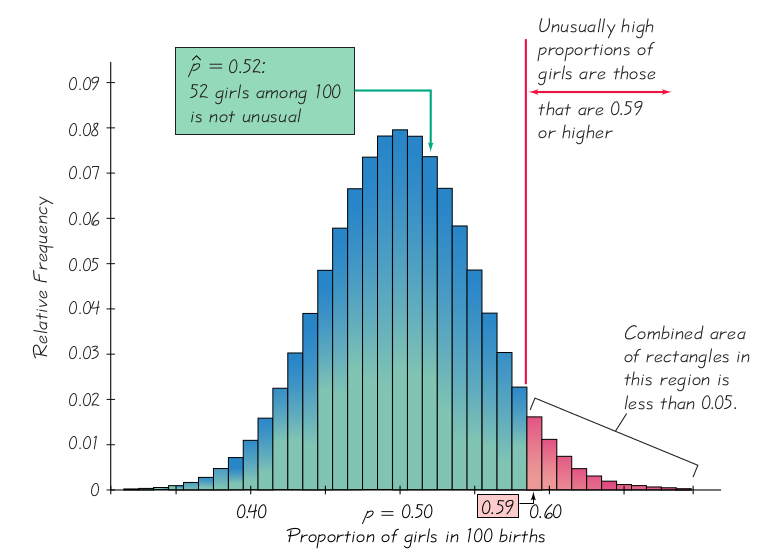
\includegraphics[width=\textwidth]{TH_I/regiao_critica1}
  \end{center}
\end{frame}

\begin{frame}{Rejeitar hipóteses}
  \begin{itemize}
  \item Ao executar um teste de hipóteses observamos se os dados
    indicam que se deve rejeitar a hipótese $H_0$.
  \item $H_0$ representa a possibilidade de observarmos o resultado ao
    acaso.
  \item Caso haja evidências para que $H_0$ seja rejeitada,
    ``assumimos'' que a $H_1$ deve ser verdadeira.
  \item Mas isso não significa que $H_0$ seja falsa e $H_1$ seja verdadeira!
  \end{itemize}
\end{frame}

\subsection{Significância}

\begin{frame}{Tipos de erros em testes de hipóteses}
  \begin{definition}
    Um \alert{erro do tipo I} ocorre se a hipótese nula for rejeitada
    quando é verdadeira.
  \end{definition}
  \begin{definition}
    Um \alert{erro do tipo II} ocorre se a hipótese não for rejeitada
    quando for falsa.
  \end{definition}
\end{frame}

\begin{frame}{Tipos de erros em testes de hipóteses}
  \begin{tabular}{c||c|c}
    Decisão & $H_0$ é verdadeira & $H_0$ é falsa \\
    \hline
    \hline
    Não rejeitar $H_0$ & Decisão correta & Erro do tipo II\\
    \hline
    Rejeitar $H_0$ & Erro do tipo I & Decisão correta\\
  \end{tabular}
\end{frame}

\begin{frame}{Rejeitar hipóteses}
  \begin{block}{Importante}
    Observe que o teste de hipótese nunca deve \alert{aceitar} uma
    hipótese nula, apenas rejeitá-la ou deixar de rejeitá-la.
  \end{block}
\end{frame}

\begin{frame}{Nível de significância}
  \begin{definition}
    O \alert{nível de significância} de um teste de hipótese é sua
    probabilidade máxima admissível para cometer um erro do tipo
    I. Ele é denotado por $\alpha$.
  \end{definition}
  \begin{definition}
    A probabilidade de se cometer um erro do tipo II é denotada por
    $\beta$.
  \end{definition}
  % \begin{itemize}
  % % \item O valor $1-\beta$ é chamado o \alert{poder do teste}.
  % % \item Devemos controlar o erro do tipo I, isto é, 
  % % \item Quando você decresce $\alpha$, você provavelmente aumentará $\beta$.
  % \end{itemize}
\end{frame}

\subsection{Região crítica}

\begin{frame}{Identificando a região crítica}
  \begin{itemize}
  \item Para identificar a região crítica (ou região de rejeição) do
    teste, devemos observar se o teste é unicaudal (à esquerda ou à
    direita) ou bicaudal.
  \item Se $H_1$ é do tipo $\ne$, o teste é bicaudal (ou bilateral).
  \item Se $H_1$ é do tipo $<$, o teste é unicaudal (ou unilateral) à esquerda.
  \item Se $H_1$ é do tipo $>$, o teste é unicaudal à direita.
  \end{itemize}
\end{frame}

\begin{frame}{Identificando a região crítica}
  \begin{center}
    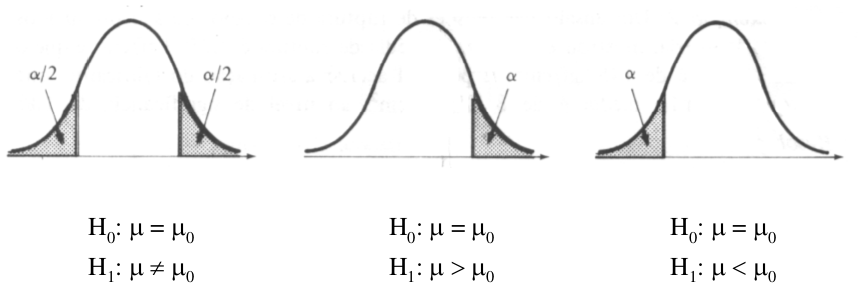
\includegraphics[width=\textwidth]{TH_I/regiao_critica2}
  \end{center}
\end{frame}

\begin{frame}{Decisão}
  \begin{itemize}
  \item Veremos a seguir uma estatística de teste para cada tipo de teste.
  \item Calculamos a estatística de teste e verificamos se esta está
    dentro da região crítica
  \item Se a estatística de teste estiver dentro da região crítica,
    devemos rejeitar $H_0$
  \item Caso contrário, não devemos rejeitar $H_0$.
  \end{itemize}
\end{frame}

\section{Testes de Hipóteses para proporções}

\subsection{Estatística de teste}

\begin{frame}{Estatística de teste}
  Em um teste de proporções, devemos considerar:
  \begin{itemize}
  \item $n$ = tamanho da amostra
  \item $\hat{p}$ = proporção na amostra
  \item $p$ = proporção na população
  \item $q=1-p$
  \item A estatística de teste para uma proporção é
    \begin{displaymath}
      z = \frac{\hat{p} - p}{\sqrt{\frac{pq}{n}}}
    \end{displaymath}
  \end{itemize}
\end{frame}

\subsection{Exemplos}

\begin{frame}{Exemplo}
  \begin{example}
    Estudos sobre mortalidade de homens com idade superior a 65 anos
    de uma cidade mostram que 4\% deles morrem dentro de um ano. Num
    grupo de 1000 indivíduos selecionados dessa população, 60 morreram
    no período de um ano. Suspeita-se de que houve um aumento da
    mortalidade anual nessa população.
  \end{example}
\end{frame}

\begin{frame}{Exemplo}
  \begin{block}{Solução}
    \begin{itemize}
    \item Hipóteses
      \begin{displaymath}
        H_0: p=0.04
      \end{displaymath}
      \begin{displaymath}
        H_1: p>0.04
      \end{displaymath}
    \item Região crítica: à direita de $z_{0.05} = \alert{1.645}$ (ou seja,
      qualquer $z>z_{0.05}$).
    \item Dados
      \begin{displaymath}
        n=1000, \hat{p} = 0,06
      \end{displaymath}
    \item Estatística de teste
      \begin{displaymath}
        z = \frac{0.06 - 0.04}{\sqrt{\frac{0.04 \times (1-0.04)}{1000}}} = \alert{3.32}
      \end{displaymath}
    \end{itemize}
  \end{block}
\end{frame}

\begin{frame}{Exemplo}
  \begin{itemize}
  \item Comparando $z$ e $z_{0.05}$ observamos que $3.32>1.645$.
  \item Como a estatística de teste está dentro da região crítica,
    rejeitamos $H_0$ ao nível de significância de 5\%.
  \item Conclusão: rejeitamos a hipótese de que a proporção de idosos
    que morrem por ano nessa cidade é igual a 4\%, em favor da
    hipótese de que essa proporção é maior 4\%, ao nível de
    significância de 5\%
  \end{itemize}
\end{frame}

\section{Testes de Hipóteses para a média}

\subsection{Estatística de teste}

\begin{frame}{Estatística de teste}
  \begin{itemize}
  \item Em um teste para a média $\mu$, devemos observar o tamanho da amostra.
  \item Se a amostra é grande, fazemos o teste Z (valor crítico $z_c$)
    com a estatística de teste:
    \begin{displaymath}
      z = \frac{\bar{x} - \mu}{\frac{s}{\sqrt{n}}}
    \end{displaymath}
  \item Se a amostra for pequena, fazemos o teste t (valor crítico
    $t_{(gl,\alpha)}$) com a estatística de teste:
    \begin{displaymath}
      t = \frac{\bar{x} - \mu}{\frac{s}{\sqrt{n}}}
    \end{displaymath}
  \end{itemize}
\end{frame}

\subsection{Exemplos}

\begin{frame}{Exemplo 1}
  \begin{example}
    Um método padrão para identificação de bactérias em hemoculturas
    vem sendo utilizado há muitos anos e seu tempo médio de execução
    (desde a etapa de preparo das amostras até a identificação do
    gênero e espécie) é de 40.5 horas. Um microbiologista propôs uma
    nova técnica que ele afirma ter menor tempo de execução que o
    método padrão. A nova técnica foi aplicada em uma amostra de 18
    hemoculturas e para cada uma mediu-se o tempo de execução. A média
    amostral foi 39.42 horas e o desvio padrão amostral foi 1,96
    horas.
  \end{example}
\end{frame}

\begin{frame}{Exemplo 1}
  \begin{itemize}
  \item Para testar essa hipótese usaremos o teste t pois a amostra é
    pequena ($n=18$) com \alert{$gl=17$} graus de liberdade.
  \item Como o teste é unicaudal (à esquerda), consultamos a tabela para a
    significância $\alpha = 0.05$.
  \item Consultando a tabela t, encontramos o valor crítico
    \alert{$t_{(17,0.05)} = 1.74$}.
  \item Após calcular a estatística de teste, devemos comparar com o
    valor crítico $t_c$ para verificar se ela está contida na região
    de rejeição.
  \end{itemize}
\end{frame}

\begin{frame}{Exemplo 1}
  \begin{block}{Solução}
    \begin{itemize}
    \item Hipóteses
      \begin{displaymath}
        H_0: \mu = 40.5
      \end{displaymath}
      \begin{displaymath}
        H_1: \mu < 40.5
      \end{displaymath}
    \item Região crítica: $t < -t_{(17,0.05)}$(ou seja, qualquer
      \alert{$t< -1.74$}).
    \item Dados
      \begin{displaymath}
        n=18, \bar{x} = 39.42, s=1.96
      \end{displaymath}
    \item Estatística de teste
      \begin{displaymath}
        t = \frac{39.42 - 40.5}{\frac{1.96}{\sqrt{18}}} = \alert{-2.34}
      \end{displaymath}
    \end{itemize}
  \end{block}
\end{frame}

\begin{frame}{Exemplo 1}
  \begin{itemize}
  \item O valor $t=-2.34$ está dentro da região crítica ($t=-2.34 < -1.74$).
  \item Como a estatística de teste está dentro da região crítica,
    rejeitamos $H_0$ ao nível de significância de 5\%.
  \item Conclusão: Rejeita-se a hipótese de que o tempo médio de
    execução do novo método é igual a 40.5 horas, em favor da hipótese
    de que ele é menor do que 40.5 horas, ao nível de significância de
    5\%
  \end{itemize}
\end{frame}

\begin{frame}{Exemplo 2}
  \begin{example}
    Uma indústria farmacêutica especifica que em certo analgésico a
    quantidade média de ácido acetil salicílico deve ser 5.5 gramas
    por comprimido. A indústria suspeita que houve problemas na
    produção de um determinado lote e que, nesse lote, a quantidade
    média dessa substância está diferente da especificada. Para
    verificar essa suspeita, a indústria selecionou uma amostra
    aleatória de 40 comprimidos desse lote, observando uma quantidade
    média de ácido acetil salicílico igual a 5.2 gramas e um desvio
    padrão de 0.7 gramas.
  \end{example}
\end{frame}

\begin{frame}{Exemplo 2}
  \begin{itemize}
  \item Para testar essa hipótese usaremos o teste Z pois a amostra é
    grande ($n=40$).
  \item O teste é bicaudal, portanto consultamos a significância
    \alert{$\frac{\alpha}{2} = 0.025$}.
  \item Consultando a tabela Z, encontramos o valor crítico
    \alert{$z_{0.025} = 1.96$}.
  \item Após calcular a estatística de teste, devemos comparar com o
    valor crítico $z_c$ para verificar se ela está contida na região
    de rejeição.
  \end{itemize}
\end{frame}

\begin{frame}{Exemplo 2}
  \begin{block}{Solução}
    \begin{itemize}
    \item Hipóteses
      \begin{displaymath}
        H_0: \mu = 5.5
      \end{displaymath}
      \begin{displaymath}
        H_1: \mu \ne 5.5
      \end{displaymath}
    \item Região crítica: $z<-z_{0.025}$ ou $z>z_{0.025}$ (ou seja,
      \alert{$z<-1.96$ ou $z>1.96$}).
    \item Dados
      \begin{displaymath}
        n=40, \bar{x} = 5.2, s = 0.7
      \end{displaymath}
    \item Estatística de teste
      \begin{displaymath}
        z = \frac{5.2 - 5.5}{\frac{0.7}{\sqrt{1000}}} = \alert{-2.71}
      \end{displaymath}
    \end{itemize}
  \end{block}
\end{frame}

\begin{frame}{Exemplo 2}
  \begin{itemize}
  \item O valor $z=-2.71$ está dentro da região crítica ($z=-2.71 < -1.96$).
  \item Como a estatística de teste está dentro da região crítica,
    rejeitamos $H_0$ ao nível de significância de 5\%.
  \item Conclusão: rejeitamos a hipótese de que a quantidade média de
    ácido acetil salicílico (gramas por comprimido) de certo
    analgésico é igual a 5.5 gramas ao nível de significância de 5\%
  \end{itemize}
\end{frame}

\begin{frame}{Bônus: Intervalo de Confiança}
  \begin{itemize}
  \item Nessa situação, podemos usar o intervalo de confiança para
    realizar o teste de hipóteses, pois a hipótese alternativa é
    bilateral.
  \item Como queremos um teste a 5\% de significância, calcularemos um
    intervalo de 95\% de confiança para a quantidade média de ácido
    acetil salicílico, por comprimido.
  \end{itemize}
\end{frame}

\begin{frame}{Exemplo 2 (a revanche)}
  \begin{example}
    \begin{columns}
      \begin{column}{5cm}
        \begin{itemize}
        \item $IC_{0.95} = (\bar{x} \pm E)$
        \item $1-\alpha = 0.95$
        \item $\alpha = 0.05$
        \item $\frac{\alpha}{2} = 0.025$
        \item $z_c = z_{0.025} = 1.96$
        \end{itemize}
      \end{column}
      \begin{column}{5cm}
        \begin{itemize}
        \item $IC_{0.95} = (5.2 \pm 1.96 \times \frac{0.7}{\sqrt{40}})$
        \item $IC_{0.95} = (5.2 \pm 0.2)$
        \item $IC_{0.95} = \alert{(5.0 , 5.4)}$
        \end{itemize}
      \end{column}
    \end{columns}
  \end{example}

  Lembrete da margem de erro: $E = z_c \times\frac{s}{\sqrt{n}}$
\end{frame}

\begin{frame}{Interpretação do IC}
  \begin{block}{Interpretação}
    A quantidade média de ácido acetil salicílico, por comprimido,
    está entre 5,0 e 5,4 gramas, com 95\% de confiança.
  \end{block}
  \begin{itemize}
  \item Teste de hipóteses baseado no intervalo de confiança: o valor
    5.5 não pertence ao intervalo de 95\% de confiança para a
    quantidade média de ácido acetil salicílico, por comprimido.
  \item Conclusão: rejeitamos a hipótese de que a quantidade média de
    ácido acetil salicílico de certo analgésico é igual a 5.5 gramas
    ao nível de significância de 5\%.
  \end{itemize}
\end{frame}
\section{Resumo}

\begin{frame}{Resumo}
  Para executar um teste de hipóteses, é necessário:
  \begin{enumerate}
  \item Formular a hipótese a ser testada e a hipótese nula, e
    escrevê-las em linguagem simbólica ($H_0$ e $H_1$)
  \item Decidir qual o tipo de teste (unicaudal à esquerda, unicaudal
    à direita ou bicaudal)
  \item Determinar a distribuição a ser usada e calcular a estatística
    de teste
  \item Verificar se esta está contida na região de rejeição e decidir
    se há evidências para rejeitar a hippótese $H_0$.
  \end{enumerate}
\end{frame}

\end{document}
